\documentclass[12pt]{article}
\usepackage[polish]{babel}
\usepackage[utf8]{inputenc}
\usepackage{tikz}
\usetikzlibrary{trees}
\usepackage{graphicx}
\graphicspath{ {./images/} }
\begin{document}

\begin{flushright}

Laboratoria: piatek, 8:00

Grupa: 13

Informatyka Wydział informatyki i telekomunikacji.

\end{flushright}

\hspace{4cm}

\begin{center}

Algorytmy i Strukrury Danych

Prowadzacy:

Dominik Witczak

\end{center}

\hspace{4cm}

\begin{center}

\textbf{Sprawozdanie do \LARGE}

\hspace{2cm}

\underline{Projektu 2 drzewa binarne}

\end{center}

\hspace{30cm}

\begin{flushright}

Autor:

Marcin Wrzaskowski

nr indeksu:

160329

\end{flushright}

\pagebreak

\section{Dzialanie programu: }

\subsection{Tworzenie drzewa samobalansujacego sie AVL}

\begin{center}

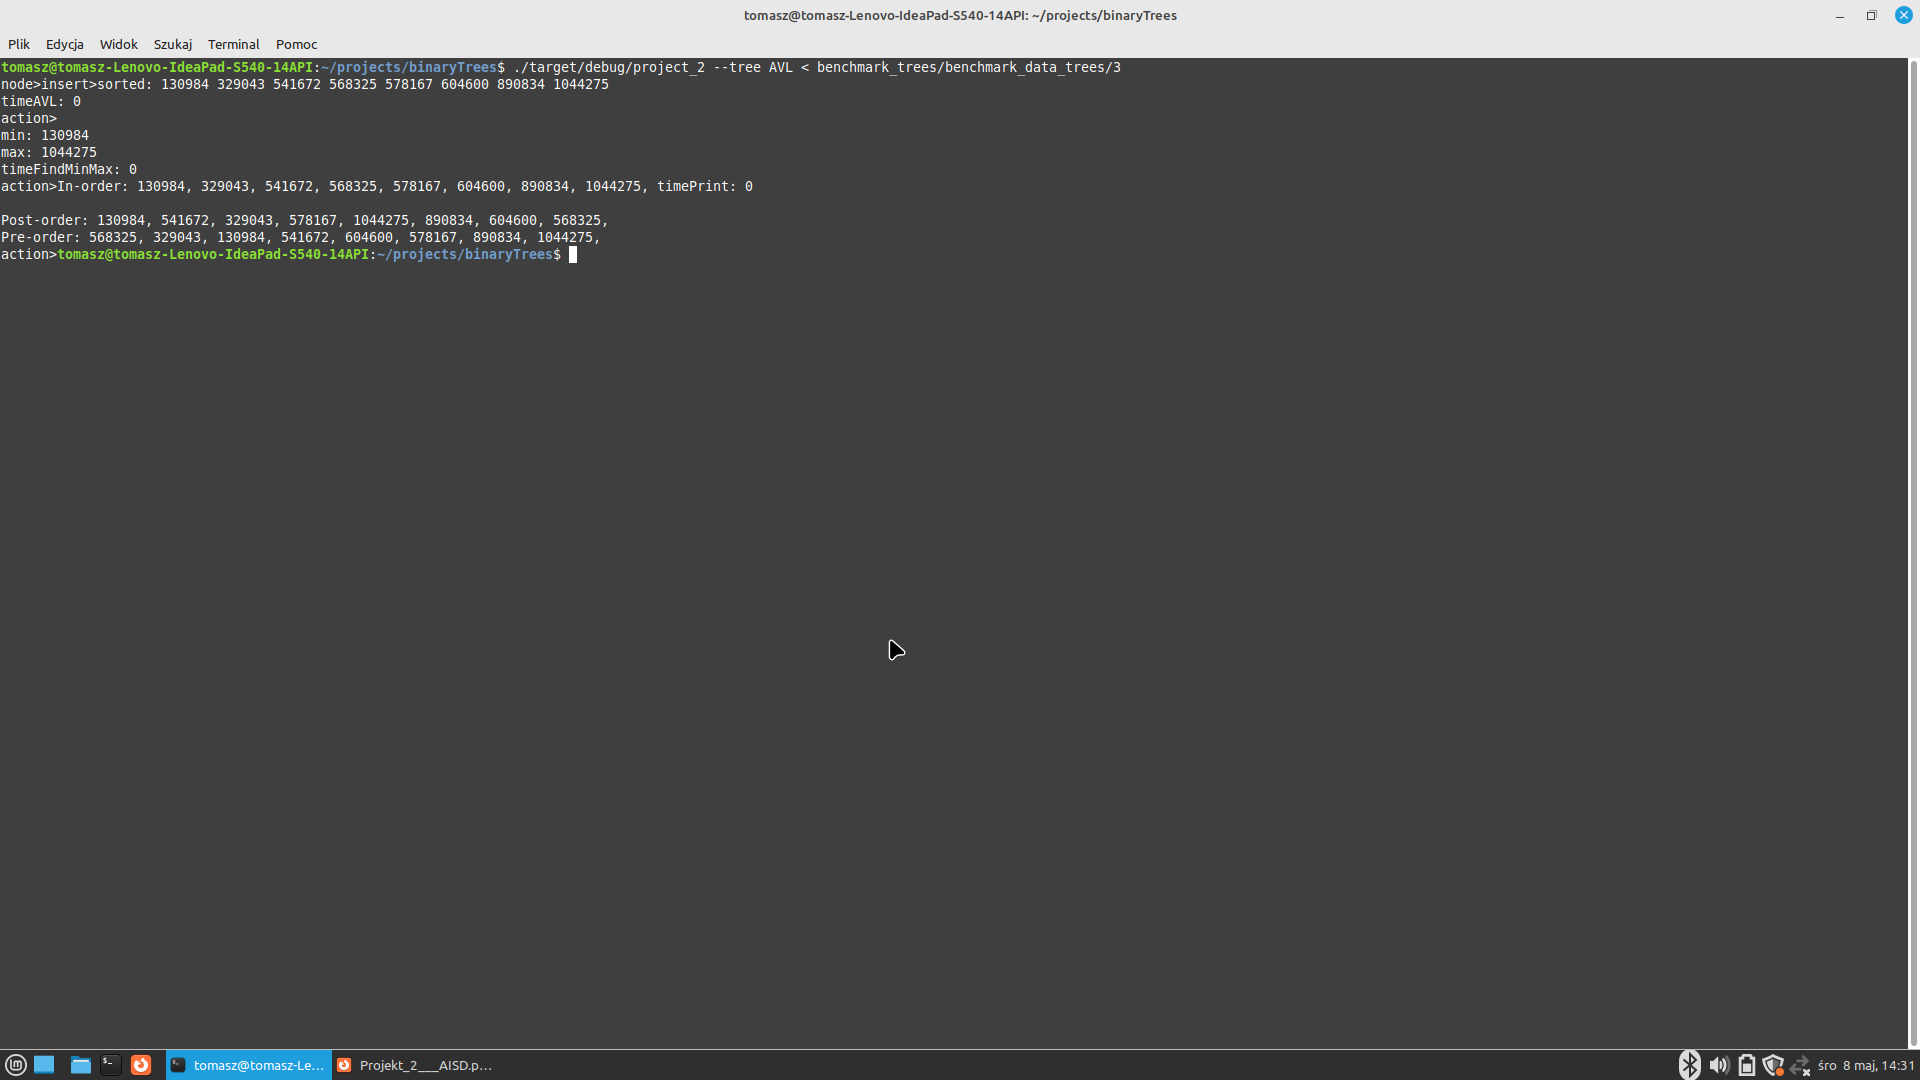
\includegraphics[scale=0.25]{createAVL.png}

\end{center}

\subsection{Tworzenie drzewa BST}

\begin{center}

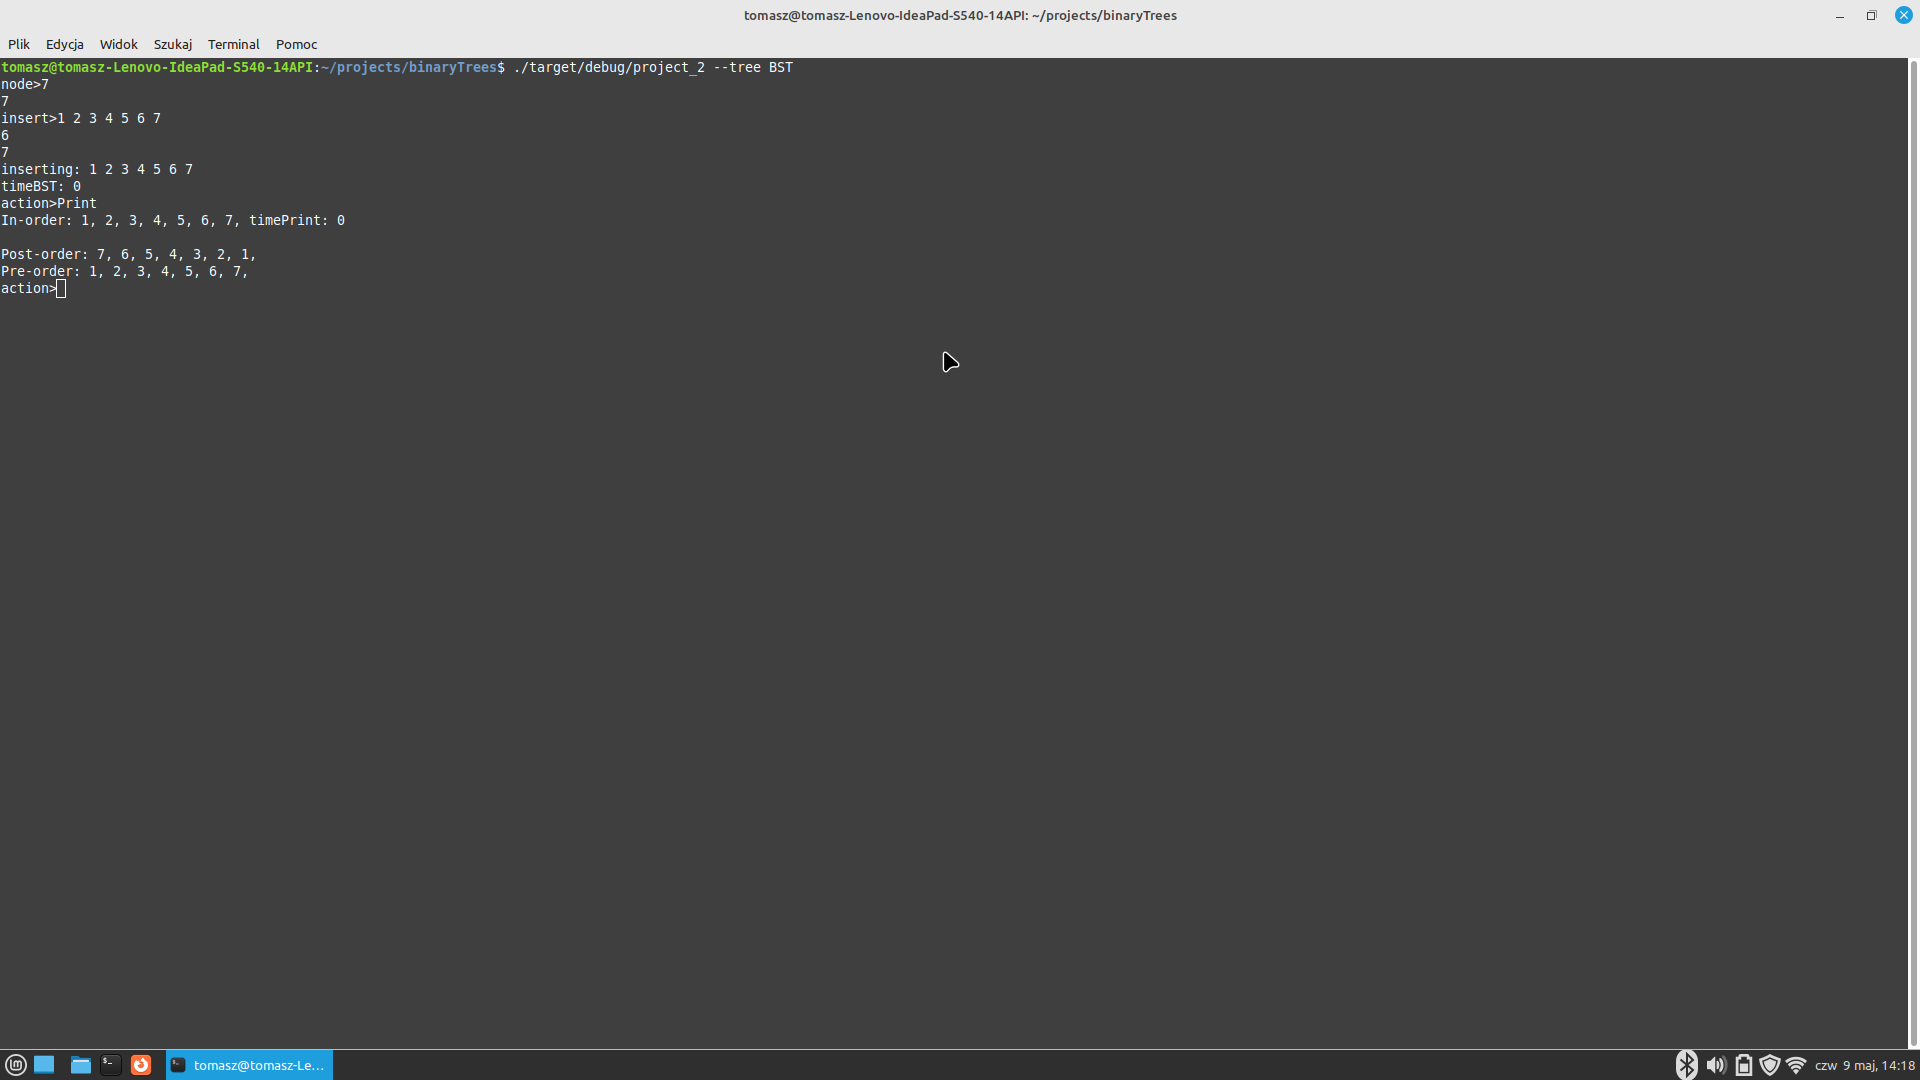
\includegraphics[scale=0.25]{createBSTNonBalanced_0.png}

\end{center}

\subsection{Wizualizacja niezbalansowanego drzewa BST}

\begin{center}

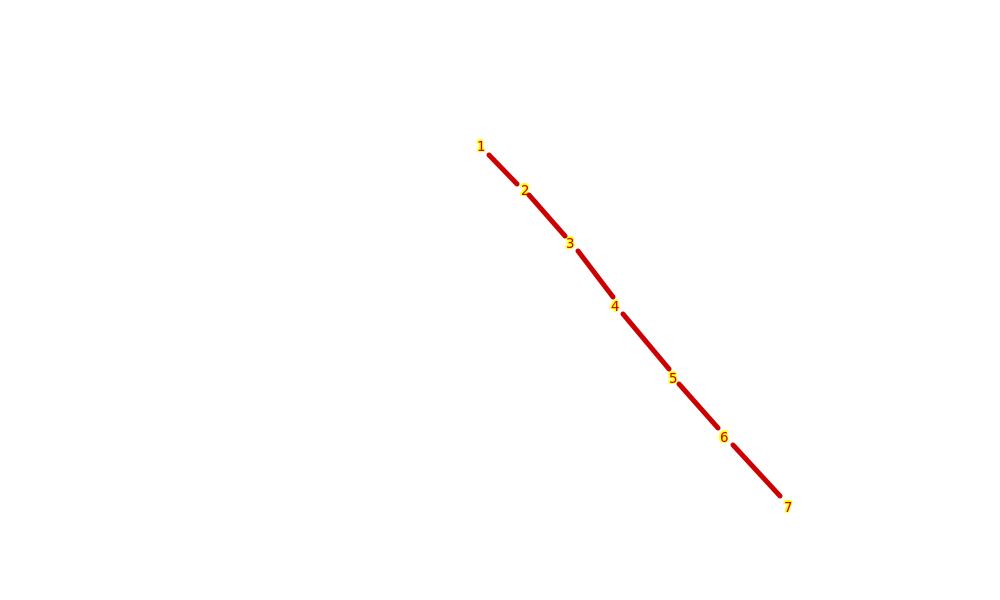
\includegraphics[scale=0.5]{bst_vi.png}	 

\end{center}

\section{Wykresy zależności $ t = f(n) $}

\subsection{Skala liniowa: }

\begin{center}

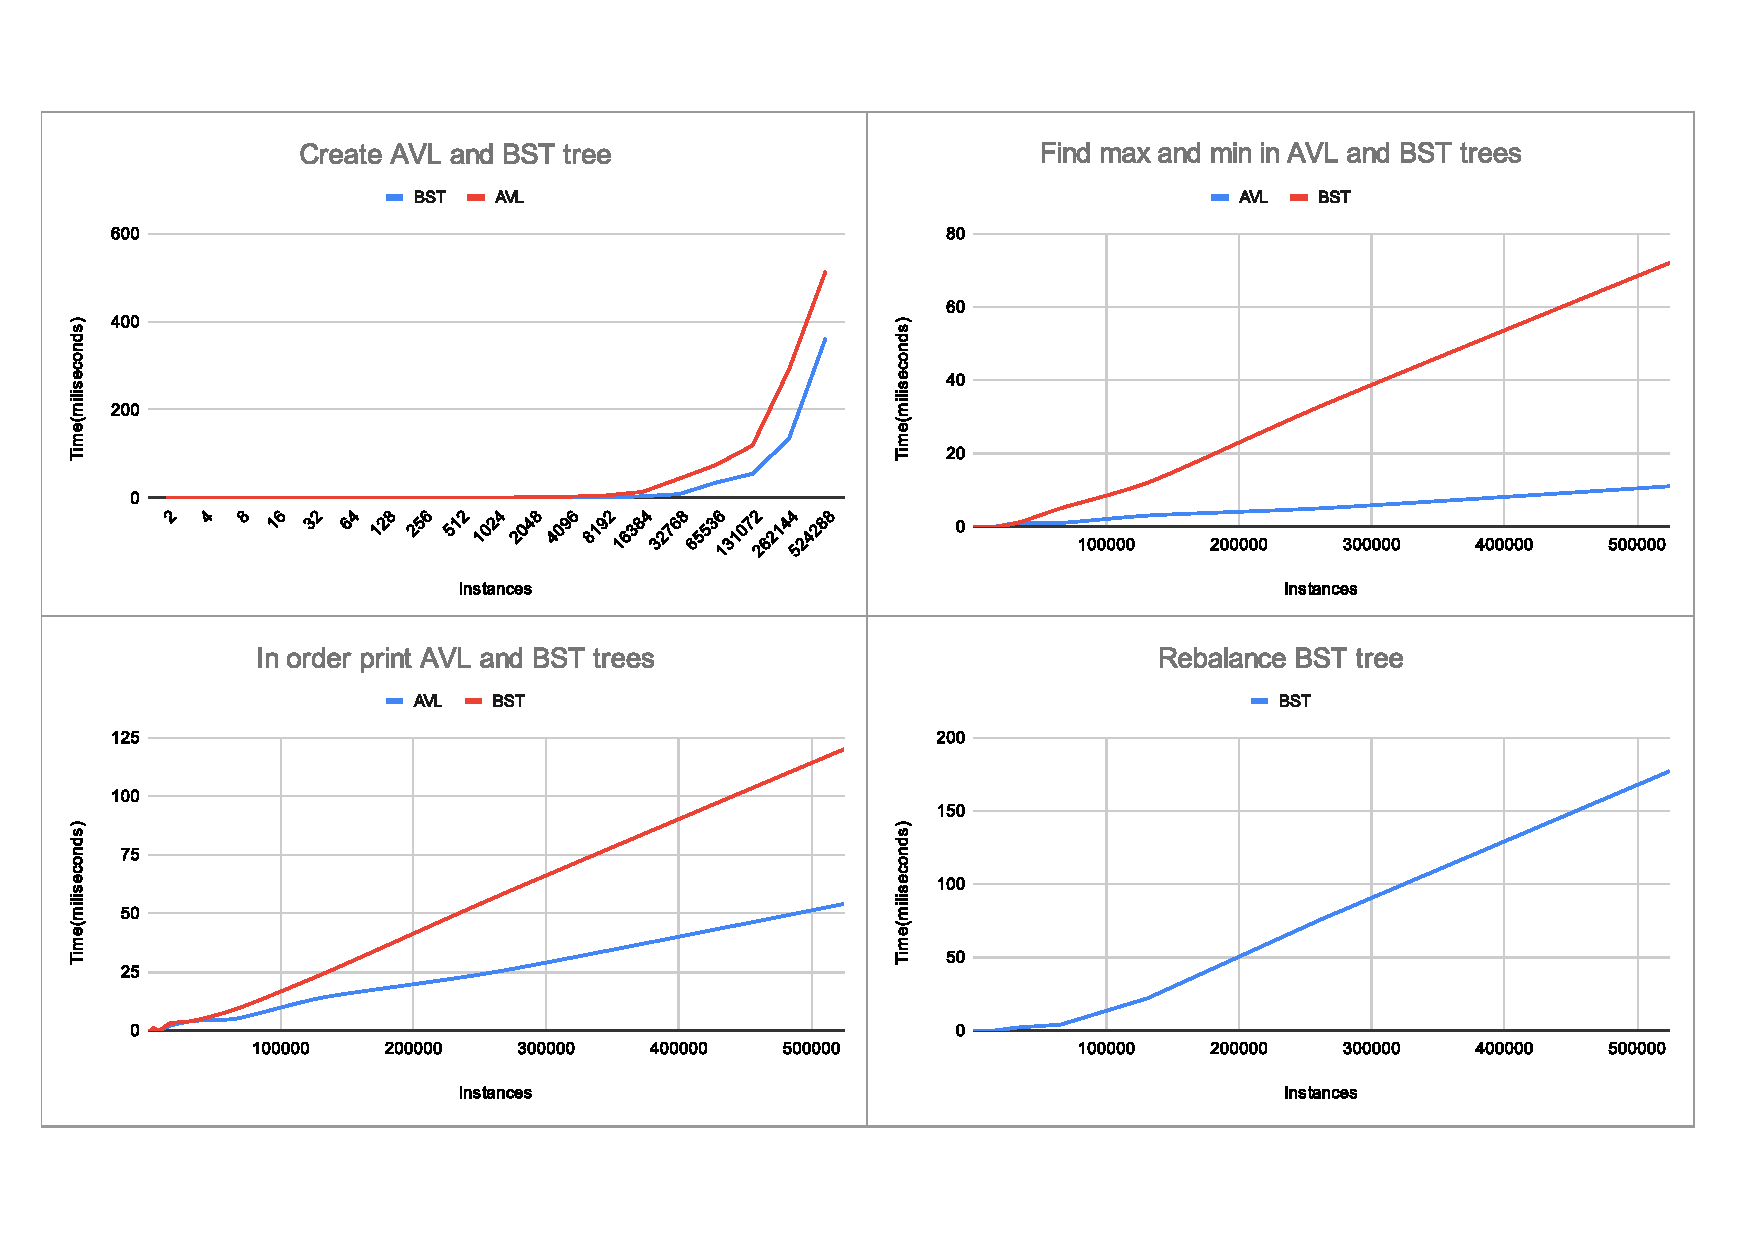
\includegraphics[width=\linewidth]{wykresy_obok_1.pdf}

\end{center}

\subsection{Skala logarytmiczna: }

\begin{center}

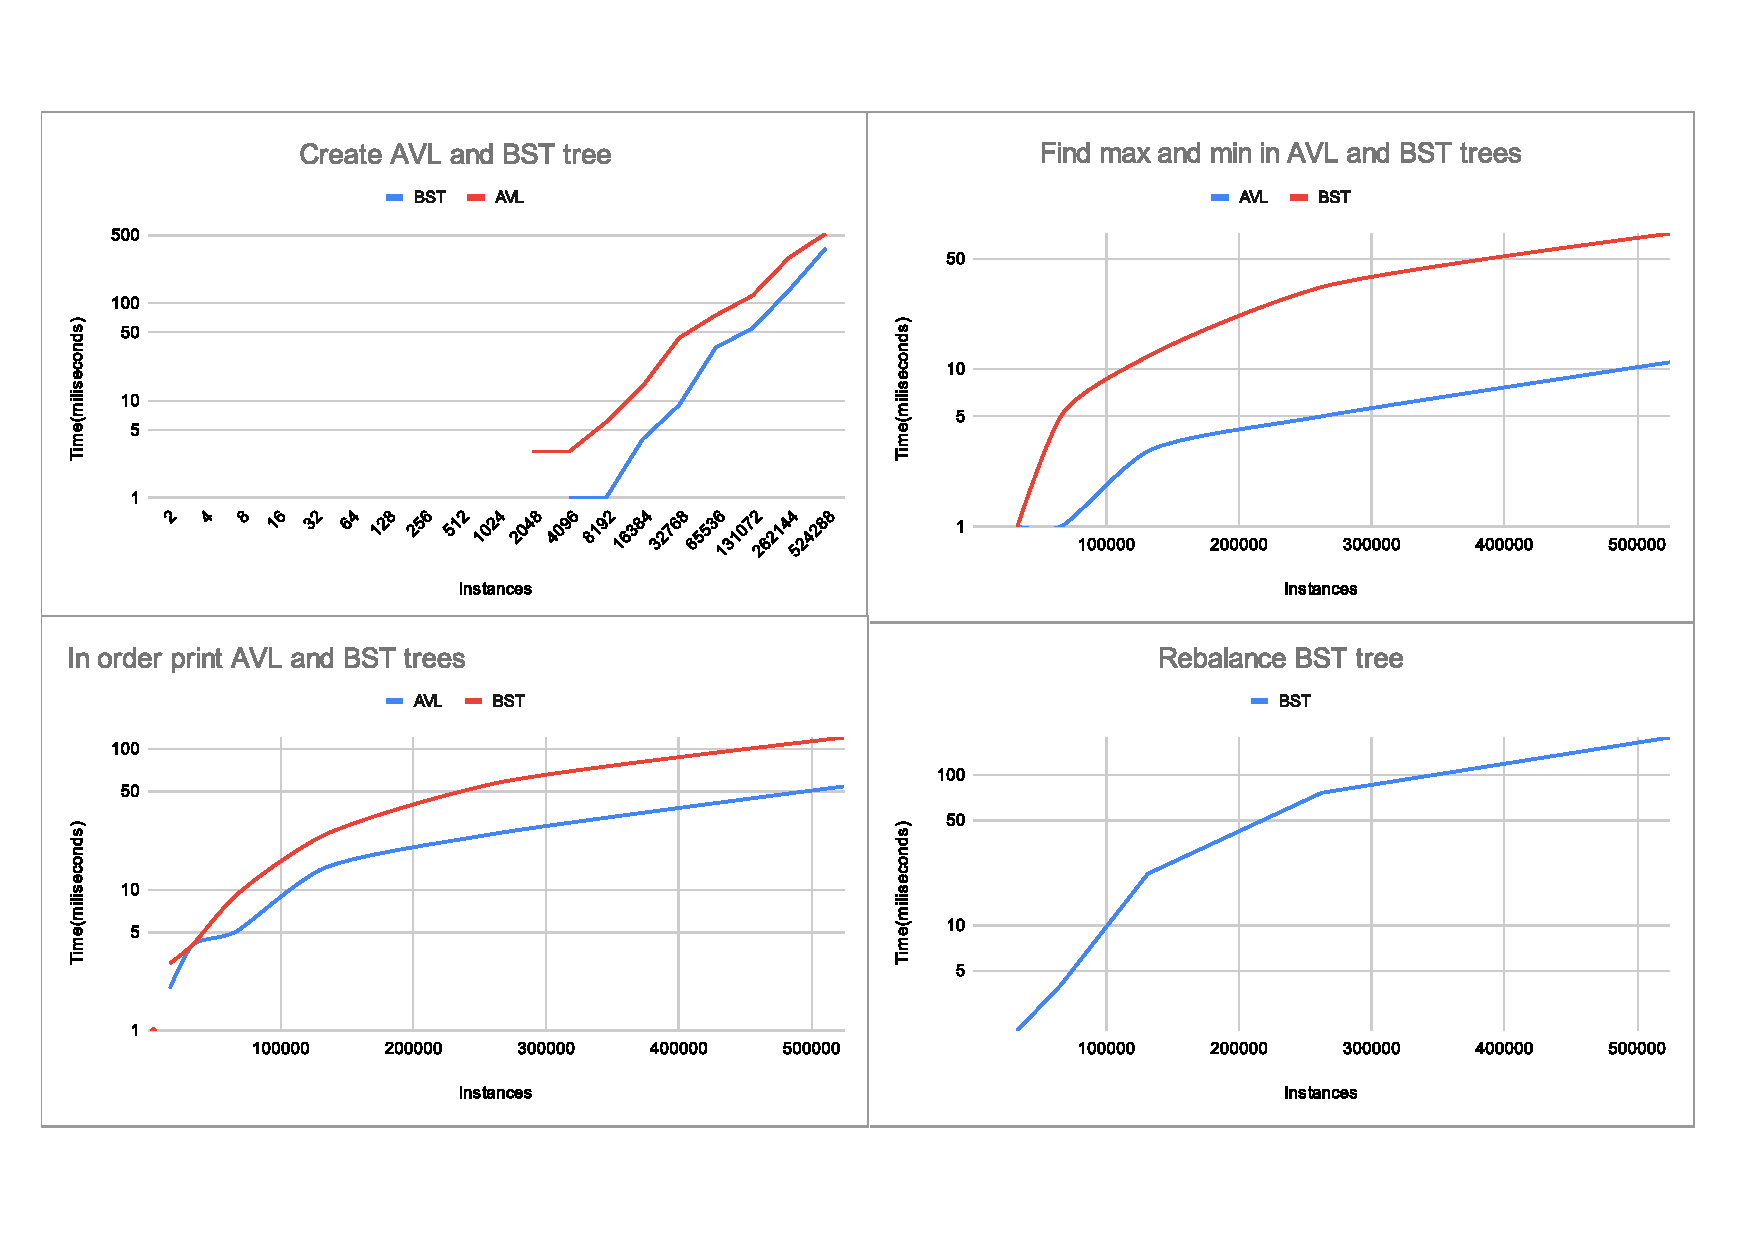
\includegraphics[width=\linewidth]{wykresy_obok_0.pdf}

\end{center}

\section{Podsumowanie: }

Nauczyłem sie

\begin{enumerate}

	\item
	      Tworzyc drzewa AVL i BST.
	\item
		  Implementowac algorytmy ktore operuja na tych strukturach.
	\item
		  O drzewach jako strukturach danych.
	\item
		  Jak zbalansowac drzewo BST
	\item
		  Jak znajdowac min i max
    \item
    	      Wypisywania w: in-order, pre-order, post-order.

\end{enumerate}

\begin{center}

\tableofcontents

\end{center}

\end{document}